\documentclass[aspectratio=169]{beamer}
\usetheme{uantwerpen}

\usepackage{mathtools}

% tikz
\usepackage{tikz}
\usetikzlibrary{automata,positioning,overlay-beamer-styles}

% macros
\newcommand{\always}{\mathop{\mathtt{G}}}
\newcommand{\evtly}{\mathop{\mathtt{F}}}
\newcommand{\until}{\mathrel{\mathtt{U}}}
\newcommand{\nxt}{\mathop{\mathtt{X}}}

% titlepage info
\title{Acacia-Bonsai}
\subtitle{A Modern Implementation of Downset-Based LTL Synthesis}
\author{Micha\"el Cadilhac \and \underline{Guillermo A. P\'erez}}
\date{TACAS 2023}

% outline before each section
\AtBeginSection[]
{
  \begin{frame}
    \frametitle{Outline}
    \tableofcontents[currentsection]
  \end{frame}
}

\begin{document}

\begin{frame}
	\titlepage
\end{frame}

\begin{frame}{Motivation: Safe Reactive Systems}
  \begin{block}{Reactive systems}
    These are systems that interact with their environment in a
    \alert{continuous} fashion, i.e. nonstop, and they are all around us:
    e.g. operating systems, schedulers, embedded controllers\dots
  \end{block}
  \begin{center}
    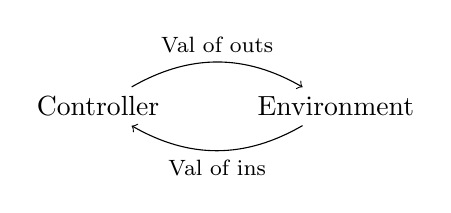
\begin{tikzpicture}
      \node (cnt) {Controller};
      \node[right= of cnt] (env) {Environment};
      \path[->,auto]
        (cnt) edge[bend left] node{\footnotesize Val of outs} (env)
        (env) edge[bend left] node{\footnotesize Val of ins} (cnt)
        ;
    \end{tikzpicture}
  \end{center}
  \pause
  \begin{block}{Safety via synthesis}
    Reactive systems are hard to design and errors can \alert{cost lives} and
    money. Hence, we would like to \alert{synthesize them} from a formal
    specification!
  \end{block}
\end{frame}

\begin{frame}{Motivation: Synthesis Competition}
  \begin{block}{SYNTCOMP}
    Since 2014, the synthesis competition SYNTCOMP gathers benchmarks and
    tools for synthesis from different specification formats:
    \begin{itemize}
      \item Safety monitors
      \item \alert{Linear temporal logic (LTL) formulas}
      \item Parity games
    \end{itemize}
  \end{block}
  \pause
  \begin{block}{LTL synthesis tools}
    Award winning tools include:
    \begin{itemize}
      \item Strix
      \item ltlsynt
      \item \alert{Acacia (no longer maintained)}
      \item \dots
    \end{itemize}
  \end{block}
\end{frame}

\section{LTL Specifications}

\begin{frame}{Linear temporal logic}
  \begin{block}{Formulas}
    Fix a set $P$ of \alert{atomic propositions}. LTL formulas are of the
    form:
    \[
      \varphi \Coloneqq a \in P \mid \varphi \land \varphi \mid
      \lnot \varphi \mid \nxt \varphi \mid \evtly \varphi \mid
      \always \varphi \mid \varphi \until \varphi
    \]
  \end{block}

  \begin{block}{Why LTL?}
    It allows to naturally specify time dependence amongst events.
    It has applications in:
    \begin{itemize}
      \item Artificial intelligence
      \item Hybrid systems and control
      \item Software engineering
      \item Bio-informatics
      \item \dots
    \end{itemize}
    It forms the basis of the \alert{Property Specification Language} (IEEE
    1850) that can be used with electronic system design languages (HDLs e.g.
    Verilog).
  \end{block}
\end{frame}

\begin{frame}{Semantics of LTL}
  \begin{block}{Semantics over words (by example)}
    ``It is always the case that if there is a request then eventually it is
    granted'':
    \[ \varphi = \bigwedge_{i=1,2} \always(\mathit{req}_i \rightarrow \evtly
    \mathit{grant}_i)\]
    \begin{itemize}
      \item
        $(\mathit{req}_1,\mathit{req}_2,\mathit{grant}_1,\overline{\mathit{grant}_2})^*
        (\overline{\mathit{req}_1},\overline{\mathit{req}_2},\overline{\mathit{grant}_1},\mathit{grant}_2)^\omega$
        \alert{satisfies} $\varphi$
        \pause
      \item
        $(\overline{\mathit{req}_1},\overline{\mathit{req}_2},\mathit{grant}_1,\mathit{grant}_2)^\omega
        \models \varphi$
    \end{itemize}
  \end{block}
  \pause
  \begin{block}{The synthesis problem}
    Does there exist a \alert{controller} $\sigma : Val(ins)^* \to Val(outs)$
    such that all outcomes consistent with $\sigma$ satisfy the specification?
    \pause
    \begin{itemize}
      \item For $\varphi$ as above, with $ins = \{req_i\}$ and $outs = \{grant_i\}$,
        \alert{yes!} ``grant all requests immediately''
    \end{itemize}
  \end{block}
\end{frame}

\section{Synthesis Algorithms}

\begin{frame}{Classical Algorithms}
  \begin{center}
    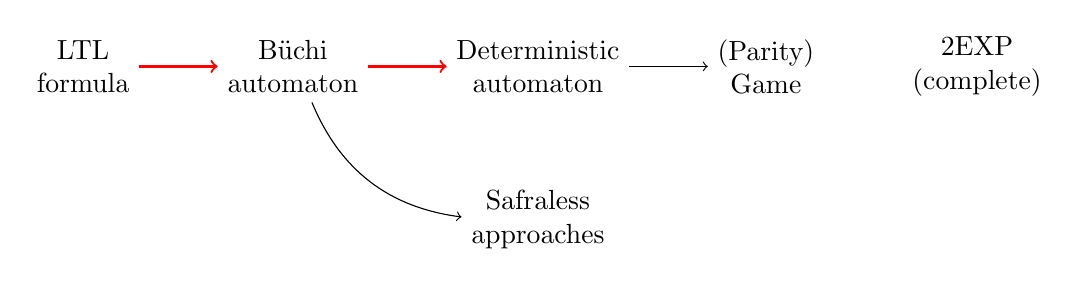
\begin{tikzpicture}
      \node[align=center] (spec) {LTL\\formula};
      \node[right= of spec,align=center] (auto) {B\"uchi\\automaton};
      \node[right= of auto,align=center] (det) {Deterministic\\automaton};
      \node[right= of det,align=center] (game) {(Parity)\\Game};
      \node[right= of game,align=center] {\alert{2EXP}\\\alert{(complete)}};
      \node[below= of det,align=center,visible on=<3->] (safraless)
        {Safraless\\approaches};
      \path[->]
        (spec) edge[thick,color=red] (auto)
        (auto) edge[thick,color=red] (det)
        (det) edge (game)
      ;
      \path[->,visible on=<3->]
        (auto) edge[bend right] (safraless)
      ;
    \end{tikzpicture}
  \end{center}
  \visible<2->{
    \begin{block}{Important optimizations}
      \begin{itemize}
        \item Normalization procedures on the LTL formula
        \item On-the-fly construction of the deterministic automaton (and game)
        \item \dots
      \end{itemize}
    \end{block}
  }
\end{frame}

% 4. Safety approximation: to avoid determinization
\begin{frame}{From LTL to B\"uchi Automata: Example}
  \[ \lnot\left(\bigwedge_{i=1,2} \always(\mathit{req}_i \rightarrow \evtly
  \mathit{grant}_i)\right)\]
  %
  \pause
  %
  \begin{center}
    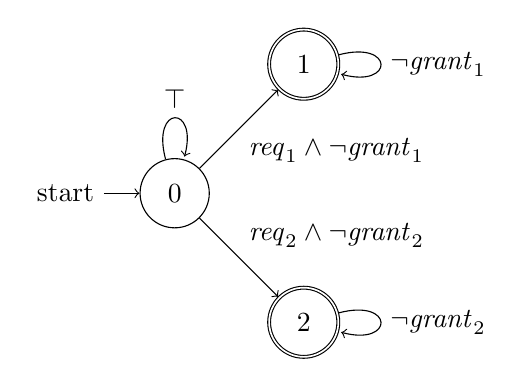
\begin{tikzpicture}
      \node[initial,state](s0){0};
      \node[state,accepting,above right= of s0](s1){1};
      \node[state,accepting,below right= of s0](s2){2};
      \path[->,auto]
        (s0) edge[loop above] node{$\top$} (s0)
        (s0) edge node[swap]{$\mathit{req}_1 \land \lnot \mathit{grant}_1$} (s1)
        (s0) edge node{$\mathit{req}_2 \land \lnot \mathit{grant}_2$} (s2)
        (s1) edge[loop right] node{$\lnot \mathit{grant}_1$} (s1)
        (s2) edge[loop right] node{$\lnot \mathit{grant}_2$} (s2)
      ;
    \end{tikzpicture}
  \end{center}
\end{frame}

\begin{frame}{Let's Play a Game}
  \begin{block}{The synthesis game}
    Let $\mathcal{A}_{\lnot \varphi}$ be the B\"uchi automaton for the
    complement of the specification $\varphi$. In each round of the game:
    \begin{enumerate}
      \item Environment chooses a valuation of ins,
      \item Controller then chooses a valuation of outs.
    \end{enumerate}
    The (infinite) outcome is \alert{winning for Controller} iff it
    satisfies $\varphi$ iff it is \emph{not} accepted by $\mathcal{A}_{\lnot
    \varphi}$.
    \begin{itemize}
      \item Non-determinism in $\mathcal{A}_{\lnot \varphi}$ makes things
        algorithmically difficult\dots
    \end{itemize}
  \end{block}
  \pause
  \begin{block}{A handicapped version of the game}
    Let $k \in \mathbb{N}$.
    \begin{itemize}
      \item Rounds of the game proceed as before.
      \item The outcome is winning for Controller iff all runs of
        $\mathcal{A}_{\lnot \varphi}$ on it reach final states \alert{at most $k$
        times}.
    \end{itemize}
  \end{block}
\end{frame}

\begin{frame}{A Concrete Game: Example}
  \begin{center}
    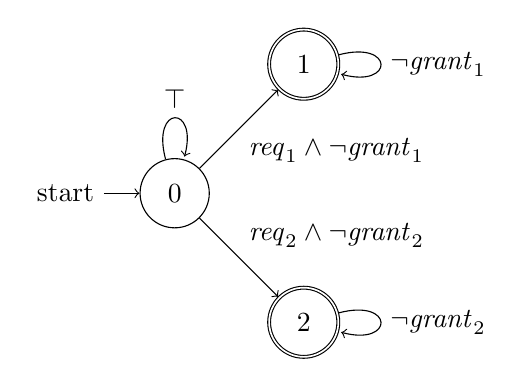
\begin{tikzpicture}
      \node[initial,state](s0){0};
      \node[state,accepting,above right= of s0](s1){1};
      \node[state,accepting,below right= of s0](s2){2};
      \path[->,auto]
        (s0) edge[loop above] node{$\top$} (s0)
        (s0) edge node[swap]{$\mathit{req}_1 \land \lnot \mathit{grant}_1$} (s1)
        (s0) edge node{$\mathit{req}_2 \land \lnot \mathit{grant}_2$} (s2)
        (s1) edge[loop right] node{$\lnot \mathit{grant}_1$} (s1)
        (s2) edge[loop right] node{$\lnot \mathit{grant}_2$} (s2)
      ;
    \end{tikzpicture}
  \end{center}
  \begin{block}{The handicap gives a conservative over-approximation}
    Controller does not grant anything, $n$ turns. Then, it grants
    everything once; grants requests immediately.
    \begin{itemize}
      \item If $k \geq n$, this is a \alert{winning strategy} for controller
        in both versions of the game.
      \item If $k < n$, this strategy is winning for the first game and
        \alert{losing for the handicapped version}.
    \end{itemize}
  \end{block}
\end{frame}

\begin{frame}{A Game Played on Vectors: k=2}
  \begin{center}
    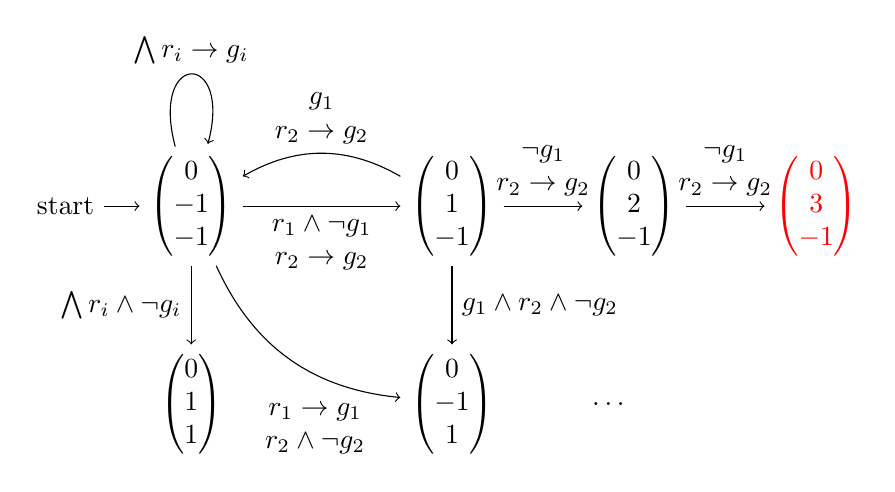
\begin{tikzpicture}
      \node[initial](v0){$\begin{pmatrix}0\\-1\\-1\end{pmatrix}$};
      \node[right=2cm of v0](v1){$\begin{pmatrix}0\\1\\-1\end{pmatrix}$};
      \node[right= of v1](v2){$\begin{pmatrix}0\\2\\-1\end{pmatrix}$};
      \node[color=red,right= of v2](v3){$\begin{pmatrix}0\\3\\-1\end{pmatrix}$};
      \node[below= of v1](v4){$\begin{pmatrix}0\\-1\\1\end{pmatrix}$};
      \node[below= of v0](v5){$\begin{pmatrix}0\\1\\1\end{pmatrix}$};
      \node[right= of v4](dots){\dots};
      \path[->,auto]
        (v0) edge[loop above] node{$\bigwedge r_i \rightarrow g_i$} (v0)
        (v0) edge node[swap,align=center]{$r_1 \land \lnot g_1$\\$r_2 \rightarrow g_2$} (v1)
        (v1) edge node[align=center]{$\lnot g_1$\\$r_2 \rightarrow g_2$} (v2)
        (v2) edge node[align=center]{$\lnot g_1$\\$r_2 \rightarrow g_2$} (v3)
        (v1) edge[bend right] node[swap,align=center]{$g_1$\\$r_2 \rightarrow g_2$} (v0)
        (v0) edge[bend right] node[swap,align=center,pos=0.9]{$r_1 \rightarrow g_1$\\$r_2 \land
        \lnot g_2$} (v4)
        (v1) edge node{$g_1 \land r_2 \land \lnot g_2$} (v4)
        (v0) edge node[swap]{$\bigwedge r_i \land \lnot g_i$} (v5)
      ;
    \end{tikzpicture}
  \end{center}
\end{frame}

\begin{frame}{Summary of the Algorithm}
  \begin{block}{From LTL to safety game}
    \begin{enumerate}
      \item Negate the specification $\varphi$
      \item Construct a B\"uchi automaton for it $\mathcal{A}_{\lnot \varphi}$
      \item Fix $k \in \mathbb{N}$, turn the handicap game into a
        \alert{safety game} played on vectors
    \end{enumerate}
  \end{block}
  \pause
  \begin{block}{Solving safety games}
    This can be done efficiently. For instance, using the \alert{UPre}
    operator on sets $S$ of vectors: 
    \begin{itemize}
      \item $s' \in \mathrm{UPre}$ if Controller cannot avoid
        reaching a state in $\mathrm{UPre}(S)$ from $s'$ in at most $1$ step
    \end{itemize}
    The set of states from which Controller has a winning strategy is exactly
    the \alert{complement} of the least fixpoint of UPre. 
  \end{block}
  \pause
  \begin{block}{On the approximation}
    There is a double-exponential $k$ such that Controller has a winning
    strategy from the initial vector iff the answer to the synthesis problem
    is \alert{yes}.
  \end{block}
\end{frame}

\section{Downsets and Antichains}

\begin{frame}{Safety is Monotonic}
  \begin{block}{Key observation}
    Let $\vec{u} \leq \vec{v}$ be states. If $\vec{u}$ is \alert{not safe} then
    $\vec{v}$ is not safe either.
    \begin{itemize}
      \item All sets computed by UPre, from the final states, are \alert{upward
        closed}!
    \end{itemize}
  \end{block}
  \pause
  \begin{block}{Solving safety games, revisited}
    We can have \alert{symbolic} versions of operators that work on
    antichains of \alert{minimal elements} to represent closed sets:
    \begin{itemize}
      \item Symbolic membership
      \item Symbolic union
      \item Symbolic intersection
      \item Symbolic UPre
    \end{itemize}
  \end{block}
\end{frame}
% 5. Downsets (a.k.a. Antichains)

\section{Acacia-Bonsai and Experiments}

% 6. Tool architecture and features

\begin{frame}{Acacia-Bonsai}
  C++20 implementation of all of the above, and more

  \begin{block}{Optimizations}
    Some based on previous antichain-based synthesis tools:
    \begin{itemize}
      \item Surely losing states
      \item Boolean states
      \item Minimizing set of input/output valuations
      \item \dots
    \end{itemize}
  \end{block}

  \pause
  \begin{block}{Antichain data structures}
    \begin{itemize}
      \item Vector
      \item Arrays (i.e. fixed size)
      \item Vectors/arrays backed by SIMD registers (data parallelism)
      \item k-d trees
      \item \dots
    \end{itemize}
  \end{block}
\end{frame}

% 7. Experimental results

\begin{frame}{Comparison}
  \centering
  \includegraphics[width=0.7\textwidth]{../doc/tacas23/img/cactus}

  Survival plot for SYNTCOMP'21 tools and Acacia-Bonsai
\end{frame}

% 8. Conclusion + future work
\begin{frame}{Conclusion}
  \begin{block}{Acacia-Bonsai}
    \begin{itemize}
      \item A modern (re)implementation of downset-based LTL realizability
      \item Soon, \alert{synthesis} and \alert{decomposition of specs}
      \item SIMD registers and advanced data structures don't help much in
        practice!
      \item All solved benchmarks can be solved with low $k$ values
    \end{itemize}
  \end{block}

  \pause

  \begin{block}{Future work}
    \begin{itemize}
      \item Try more data structures for antichains
      \item GPU instead of SIMD?
    \end{itemize}
  \end{block}
\end{frame}

\begin{frame}
  \centering
  \includegraphics[width=0.5\textwidth]{abonsai-magritte}

  An Acacia Bonsai (By R. Magritte), by Dall-E 2
\end{frame}

\end{document}
